\section{Testing and characterization method}
\label{Method}

\subsection{Noise stage}
The window size is \SI{600}{ns}. For 20kHz dark noise rate, the expected dark noise pulse number is 0.012, which means the probability of 2 or more pulse is about 0.012 of probability of 1 pulse. The maximum peak in each waveform are extracted as the noise pulse candidates.
\subsubsection{Baseline}
Due to the offset mentioned in sec~\ref{sec:setup}, the ADC value of baseline is about 950. To get baseline, the pulse area should be removed. A procedure to determine the baseline is developed, which comprised three steps and shown in Fig~\ref{fig:baseline1}
\begin{figure}[!htbp]
    \centering
    \begin{subfigure}[b]{\textwidth}
        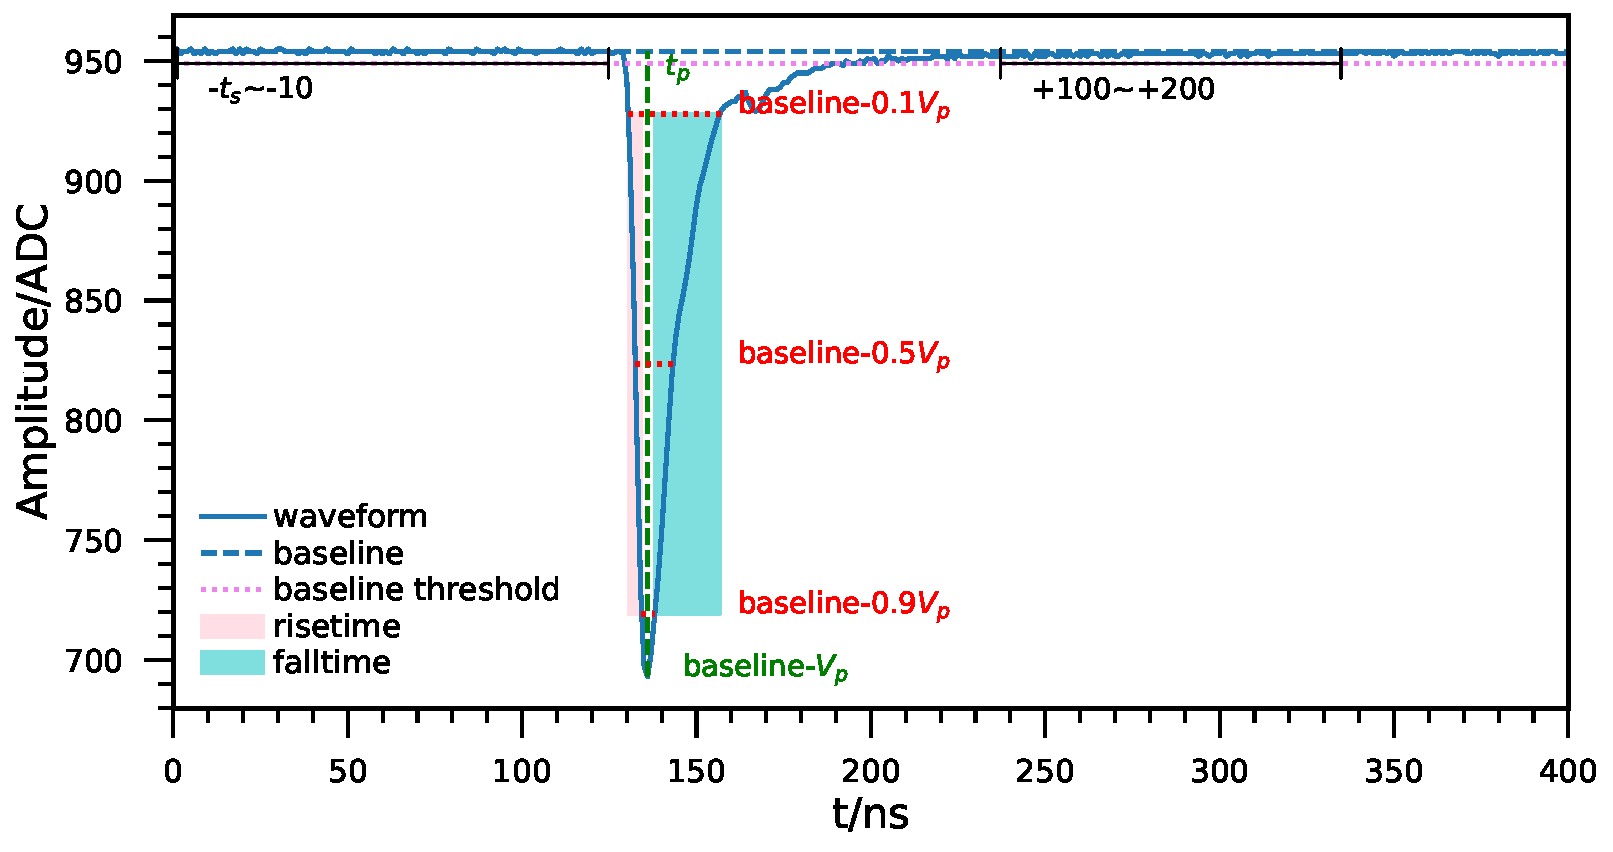
\includegraphics[width=\textwidth,page=1]{figures/result/noisebaseline697_219908_2.pdf}
        \caption{An example of waveform in noise stage}
        \label{fig:baseline1}
    \end{subfigure}
    \begin{subfigure}[b]{\textwidth}
        \includegraphics[width=\textwidth,page=3]{figures/result/noisebaseline697_219908_2.pdf}
        \caption{An example of waveform without baseline in noise stage}
        \label{fig:baseline2}
    \end{subfigure}
\end{figure}

1. An interval in the time window $[-t_s,-10]$ ($t_s\in[-200,-110]$) ns relative to pulse peak $t_p$ is selected. If $t_s<110$ when the peak is close to the start of waveform, another interval $[100,200]$ ns relative to $t_p$ is appended to expand the total interval. Average $\mu_b^0$ and standard deviation $\sigma_b^0$ of amplitudes are calculated.

2. An amplitude filter $[\mu_b^0-\max(\min(5\sigma_b^0,3),1)]$ is used to remove most of signal and reserve the baseline when $\sigma_b^0$ is small.

3. The rest amplitudes are fitted with a gaussian function G$(\mu_b^f,\sigma_b^f)$ using unbinned likelihood. $\mu_b^f$ and $\sigma_b^f$ are accurate at most time. When there exsit a large wave in the time interval selected in step1, a bias will be introduced for $\sigma_b^f$ which can be seen in Fig~\ref{fig:baselineBias2}.

4. Another amplitude filter $[\mu_b^f-\min(5\sigma_b^f,3)]$ is used to reselect the signal area and those areas are padding \SI{10}{ns} to remove rising edge and falling edge. The rest wave are used to estimate baseline $\mu_b$ and standard deviation of baseline $\sigma_b$.
\begin{figure}[!htbp]
    \centering
    \begin{subfigure}[b]{0.7\textwidth}
        % \includegraphics[width=0.8\textwidth]{figure/facility/facility.pdf}
        \caption{Peak distribution of an example PMT}%PM
        \label{fig:baselineBias1}
    \end{subfigure}
    \begin{subfigure}[b]{0.3\textwidth}
        % \includegraphics[width=0.8\textwidth]{figure/facility/facility.pdf}
        \caption{An example of waveform in noise stage}
        \label{fig:baselineBias2}
    \end{subfigure}
\end{figure}

\subsubsection{Peak and charge spectrum}
\label{sec:noisepeak}
The charge of pulses is calculated using integration in a time window $[-15, 75]$ ns relative to the peak location $t_p$ of the signal (Fig~\ref{fig:baseline2}) considering the rise time and fall time distribution. The equivalent charge $C_{\mathrm{equ}}$ is defined as the summation of the amplitude in the integration interval. Considering the input impedance is \SI{50}{\Omega}, the true charge is calculated as Equ~\eqref{equ:charge} 
\begin{equation}
    \label{equ:charge}
    C = \frac{C_{equ}}{50\Omega}
\end{equation}


The peak amplitude distribution is shown in Fig~\ref{fig:peak}
\begin{figure}[!htbp]
    \centering
    \begin{subfigure}[t]{0.45\textwidth}
        \includegraphics[width=\textwidth,page=3]{figures/result/peakcharge697.pdf}
        \caption{Charge distribution of an example PMT}%PM
        \label{fig:charge}
    \end{subfigure}
    \begin{subfigure}[t]{0.45\textwidth}
        \includegraphics[width=\textwidth,page=5]{figures/result/peakcharge697.pdf}
        \caption{ distribution of an example PMT}%PM
        \label{fig:peak}
    \end{subfigure}
    \caption{Peak and charge distribution of an example PMT}
\end{figure}
\subsubsection{Gain and single PE resolution}
There exist a long tail in charge distribution as shown in the histogram with \SI{1}{ADCns} in Fig~\ref{fig:charge}. To decrease the influence on the energy resolution, a fit interval $-30, 30$ ADCns relative to the largest count bin of histogram is used. A gaussian function G$(C_1,\sigma_{C_1})$ is used to fit the binned data via modified least-square method to get the peak of single PE. The gain $G$ is calculated as following equation
\begin{equation}
    G=\frac{C_1}{e}
\end{equation}
in which e is the charge of an electron.

The single PE resolution is defined as
\begin{equation}
    G=\frac{\sigma_{C_1}}{C_1}
\end{equation}
\subsubsection{Peak-to-valley(P/V) ratio}
A parabolic function is fitted to the vally interval as shown in Fig~\ref{fig:charge}.
The local minimum $N_v$ of charge spectrum between pedestal and SPE peak is fitted by a parabolic function. The $N_p$ is the peak fitted with gaussian function described in sec~\ref{sec:triggerpeak}.
The peak-to-valley ratio is equal to  
\begin{equation}
    P/V=\frac{N_p}{N_v}
\end{equation}
The P/V show the ability of discrimination between electronic noise and true signal. The results shows P/V of MCP PMTs are better than reference PMT.
\subsubsection{rise time, fall time and full width at half maximum(FWHM)}
The definitions of rise time, fall time and FWHM are shown in Fig~\ref{fig:waveform}($t_{10}, t_{90}$ are the time of 10\% and 90\% amplitude). Fig~\ref{fig:FWHM} shows the distribution of a PMT.
\begin{figure}
    % \includegraphics[width=0.8\textwidth]{figure/facility/facility.pdf}
    \caption{An example of FWHM in noise stage}
    \label{fig:FWHM}
\end{figure}
\subsubsection{Dark count rate}
A float threshold $V_{t}$ as shown in Fig~\ref{fig:peak} was selected as the vally of histogram of peak distributuion to discriminate the dark noise and fluctuation of baseline. The DCR equals to $\frac{N_{\mathrm{noise}}}{N_{t}}$, in which $N_{\mathrm{noise}}$ is the noise number and $N_{t}$ is the total number of waveforms.

\subsection{Laser stage}
The window size is \SI{10400}{ns} and the trigger time is at ~\SI{200}{ns} as shown in Fig~\ref{fig:triggerwaveform}. The trigger pulse are mainly centering in the time interval between [250, 350]ns dependent on the length of cable. The maximum peak are found in the window of [0, 600]ns and extract the peak position. A gaussian function G$(\mu_t^0,\sigma_t^0)$ is fit to the distribution of peak location shown in Fig~\ref{peaklocation}. A time cut $[\mu_t^0-3\sigma_t^0, \mu_t^0+3\sigma_t^0]$ is used for the waveforms dataset of each PMTs. All the characterizations are recalculated with the new time cut.

In order to yield SPE events as signal the laser intensity was adjusted to a level where only
about one out of 20 trigger signals led to a PMT signal.

\begin{figure}
    \centering
    \begin{subfigure}[b]{0.35\textwidth}
        % \includegraphics[width=0.8\textwidth]{figure/facility/facility.pdf}
        \caption{An example of waveform in laser stage}
        \label{fig:triggerwaveform}
    \end{subfigure}
    \begin{subfigure}[b]{0.35\textwidth}
        % \includegraphics[width=0.8\textwidth]{figure/facility/facility.pdf}
        \caption{peak location distribution of an example PMT}%PM
        \label{fig:peaklocation}
    \end{subfigure}
    \caption{Peak and charge distribution of an example PMT}
\end{figure}
\subsubsection{Stability of intensity of laser}
\subsubsection{Peak and charge spectrum}
\label{sec:triggerpeak}
The peak and charge calculation method are same as above in sec~\ref{sec:noisepeak}.

The peak amplitude distribution is shown in Fig~\ref{fig:triggerpeak}. The charge distribution with amplitude cut is shown in Fig~\ref{fig:triggercharge}.
\begin{figure}[!htbp]
    \centering
    \begin{subfigure}[b]{0.35\textwidth}
        % \includegraphics[width=0.8\textwidth]{figure/facility/facility.pdf}
        \caption{Peak distribution of an example PMT}%PM
        \label{fig:triggerpeak}
    \end{subfigure}
    \begin{subfigure}[b]{0.35\textwidth}
        % \includegraphics[width=0.8\textwidth]{figure/facility/facility.pdf}
        \caption{Charge distribution of an example PMT}%PM
        \label{fig:triggercharge}
    \end{subfigure}
    \caption{Peak and charge distribution of an example PMT}
\end{figure}
The results of noise and trigger methods are consist.
\subsubsection{Gain and single PE resolution}
Due to the charge distribution contains a long tail, a guassian function G$(G_1,\sigma_{G1})$ is fit to the main peak with cut between . The gain $G$ is calculated as following equation
\begin{equation}
    G=\frac{Q_1}{Q_{\mathrm{ped}}}
\end{equation}
in which $Q_{\mathrm{ped}}$ is set as 0.
\subsubsection{Peak-to-valley(P/V) ratio}
The local minimum $N_v$ of charge spectrum between pedestal and SPE peak is fitted by a parabolic function. The $N_p$ is the peak fitted with gaussian function described in sec~\ref{sec:triggerpeak}.
The peak-to-valley ratio is equal to  
\begin{equation}
    P/V=\frac{N_p}{N_v}
\end{equation}
The P/V show the ability of discrimination between electronic noise and true signal. The results shows P/V of MCP PMTs are better than reference PMT.
\subsubsection{rise time, fall time and full width at half maximum(FWHM)}
The definitions of rise time, fall time and FWHM are shown in Fig~\ref{fig:waveform}($t_{10}, t_{90}$ are the time of 10\% and 90\% amplitude). Fig~\ref{fig:FWHM} shows the distribution of a PMT.
\begin{figure}
    % \includegraphics[width=0.8\textwidth]{figure/facility/facility.pdf}
    \caption{An example of FWHM in noise stage}
    \label{fig:FWHM}
\end{figure}
\subsubsection{Transit time spread (TTS)}
The transit time spread (TTS) is the spread of photo-electron transit time (TT), which represents resolution of timing. The transit time cannot be measured directly, while the trigger time of laser and time of pulse can be measured. A relative transit time ($\mathrm{TT}_r$) is definited as the time between trigger time and $t_{10}^r$. A gaussian fuction G$(\mu_t,\mathrm{TTS}^2)$ is fitted to the distribution of $\mathrm{TT}_r$.
\subsubsection{Single electron response (SER)}
All the waveform from the the charge cut [] are align with $t_{10}^r$ and average to get the SER.
\subsubsection{Pre-pulse and after-pulse}
Pre-pulses generate due to photons hit on the MCP or the first dynode directly rather than the photocathode\cite{JUNOMassTesting}. The amplitude of pre-pulses are smaller than normal signal and appear before the main pulse. This ratio is related to the intensity of light source.
% waveform analysis
Afterpulse are generated due to the ionization of gaseous impurities between the cathode and first dynode when photo-electrons go through\cite{Coates_1973}. These ions hit back on the photocathode and generate electrons. $H^+,He^+,O^+$ are the major ions contributing to afterpulse\cite{Coates_1973}. Due to these ions are heavy than electron, the travel time is in the scale of \si{us}\footnote{The velocity of ions is about \SI{1000}{km/s} and size of PMT is about \SI{0.1}{m}, thus the transit time is about \SI{0.1}{us}}. The after pulse is calculated in a window \SIrange{300}{10000}{ns} after the main pulse.


Afterpulse is categorized into several kinds. Fig~\ref{fig:afterpulse} indicates serveral typical after-pulse peaks in time around \SI{1000}{ns} with ratio about xx\%. Considering the different mass of ions, these peaks originates from xx, xx.
\subsubsection{relative photon detection efficiency}
To measure PDE, the intensity of light and light allocation ratio of each channel need to be calibrated. For example JUNO fixed one reference PMT and other reference PMTs are circulated through all channels \cite{Wonsak_2021}. A new method is designed to reduce the number of reference PMT and combine all test runs to do calibration.  

Note $n,j,k$ ($n=0,...,N-1, j=0,...,J-1, k=0,...,K-1$) is the indicator of test run, channel of splitter and PMT. Intensity of light is $I_n$, light allocation ratio is $\alpha_j$ and photon detection efficiency is $\eta_k$. Assume $\alpha_j$s are stable among different test runs. The trigger rate of nth run, kth PMT in jth channel is
\begin{equation}
    \label{equ:pderate}
    R_{njk}=I_n\alpha_j\eta_k
\end{equation}
For convenience, 0th PMT is the reference PMT. Note $\alpha_j^0=\frac{\alpha_j}{\alpha_0}$, $\eta_k^0=\frac{\eta_k}{\eta_0}$, $I_n^0=I_n\alpha_0\eta_0$, Equ~\eqref{equ:pderate} can be transfer to Equ~\eqref{equ:pdelograte}
\begin{equation}
    \label{equ:pdelograte}
    \mathrm{log}(R_{njk})=\mathrm{log}(I_n^0)+\mathrm{log}(\alpha_j^0)+\mathrm{log}(\eta_k^0)
\end{equation}
Equ~\eqref{equ:pdelograte} is a equation set with $NK$ equations. $I_n^0,\alpha_j^0,\eta_k^0$ are the unknown $N+K+J-2$ parameters, which can stacked into an array $X = C(\mathrm{log}(I_n^0), \mathrm{log}(\alpha_j^0),\mathrm{log}(\eta_k^0))$ ($n=0,...,N-1, j=1,...,J-1, k=1,...,K-1$). 
\begin{equation}
    \mathrm{log}(R_{njk})=DX
\end{equation}
in which $D=[D_I,D_\alpha, D_\eta]$ is a sparse matrix, $D_I[{njk},n]=1,D_\alpha[{njk},j-1]=1, D_\eta[{njk},k-1]=1$. 
In Appendix~\ref{sec:solution} there exist solution only when the  equation set